%
% 4-schnell.tex
%
% (c) 2022 Prof Dr Andreas Müller, OST Ostschweizer Fachhochschule
%
\section{Schnelle Algorithmen für die Fourier-Transformation
\label{buch:diskret:section:schnell}}
\kopfrechts{Schnelle Algorithmen}
Die Berechnung Fourier-Transformierten $\hat{f}=\mathscr{F}_nf$ eines
$n$-dimensionalen Vektors $f$ als Produkt einer $n\times n$-Matrix mit
einem Vektor benötigt $n^2$ Multiplikationen und $n(n-1)$ Additionen,
also $O(n^2)$ Operationen.
Verdoppelung der Vektorlänge führt zu einer Vervierfachung der Rechenzeit.
Für zweidimensionale Anwendungen, wie sie in der Bildverarbeitung
benötig werden, ergibt sich sogar ein Faktor 16.
Die Rechenzeit limitiert die Nützlichkeit der Fourier-Transformation
beträchtlich.
In diesem Abschnitt soll gezeigt werden, wie die in
Abschnitt~\ref{buch:diskret:section:vandermonde} hergeleitete
Faktorisierung der Vandermonde-Matrix ermöglicht, die Fourier-Transformation
in $O(n\log n)$ statt $O(n^2)$ Operationen berechnet werden kann.

%
% Primfaktorisierung von $n$
%
\subsection{Primfaktorisierung von $n$
\label{buch:diskret:schnell:subsection:primfaktorisierung}}
Der Fundamentalsatz der Arithmetik besagt, dass jede natürlich Zahl $n$
eine bis auf die Reihenfolge der Faktoren eindeutige Zerlegung in
Primfaktoren
\begin{equation}
n = p_1^{n_1} p_2^{n_2} \cdots p_k^{n_k}
\label{buch:diskret:schnell:eqn:pfakt}
\end{equation}
hat.
Die Faktorisierung kann wie folgt rekursiv gefunden werden.
Sei $p_1,p_2,p_3,\dots$ die aufsteigende Folge aller Primzahlen, die
$\le \sqrt{n}$ sind.
Jetzt werden der Reihe nach alle Primzahlen $p_l$ daraufhin getestet,
ob sie $n$ teilen.
Wenn kein Teiler gefunden wird, dann ist $n$ eine Primzahl und kann
nicht weiter faktorisiert werden.
Ist $p_l\mid n$ ein Teiler, dann ist $m=n/p_l$ eine natürlich Zahl
und die Zahl $n$ kann als $n=p_l\cdot m$ faktorisiert werden.

Aus der Primfaktorisierung~\eqref{buch:diskret:schnell:eqn:pfakt}
von $n$ lasen sich alle möglichen Faktorisierungen ablesen.
Zwei Faktor $m'$ und $m''$ haben ihre eigenen Faktorzerlegungen
\[
m'= p_1^{n_1'}p_2^{n_2'}\cdots p_k^{n_k'}
\qquad\text{und}\qquad
m''= p_1^{n_1''}p_2^{n_2''}\cdots p_k^{n_k''}.
\]
Damit $m'\cdot m''=n$ gilt, müssen für die Exponenten die Gleichungen
\[
n_1=n_1'+n_1'',\quad
n_2=n_2'+n_2'',\quad\dots\quad
n_k=n_k'+n_k''
\]
gelten.
Da alle $n_i'$ und $n_i''$ natürliche Zahlen sein müssen, muss
\[
0\le n_i'\le n_i
\]
für alle $i=1,\dots,k$ sein.
Es gibt daher
\[
(n_1+1)(n_2+1)\dots(n_k+1)
\]
Faktorisierungen der Form
\[
n
=
\underbrace{
p_1^{n_1'}p_2^{n_2'}\cdots p_k^{n_k'}
}_{\displaystyle m'}
\underbrace{
p_1^{n_1-n_1'}p_2^{n_2-n_2'}\cdots p_k^{n_k-n_k'}
}_{\displaystyle m''}
\]

Für jede mögliche Faktorisierung $n=m'\cdot m''$ gibt es nach
Satz~\ref{buch:diskret:vandermonde:satz:fourierfaktorisierung}
der Fourier-Transformation $\mathscr{F}$ in zwei Faktoren
\[
\mathscr{F}_n
=
\frac{1}{m'} A(m',m'',\omega) (I_{m'}\otimes \mathscr{F}_{m''})
\]
mit $\omega=e^{-2\pi i/n}$.

%
% Faktorzerlegung der Fourier-Transformation
%
\subsection{Volle Faktorzerlegung der Fourier-Transformation
\label{buch:diskret:schnell:subsection:fourierfaktorisierung}}
\begin{figure}
\centering
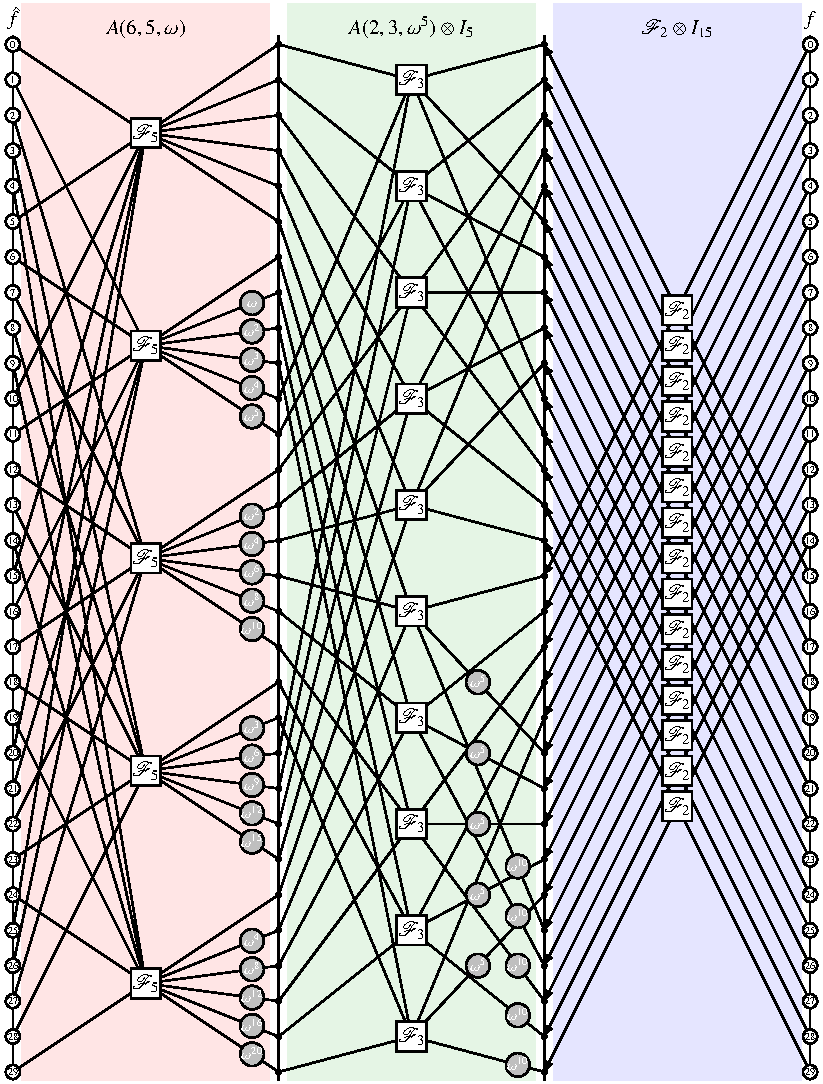
\includegraphics{chapters/060-diskret/images/f30.pdf}
\caption{Faktorisierung der Fourier-Transformation
$\mathscr{F}_{30}$ in die Faktoren
$\mathscr{F}_{30}=A(5,6,\omega)\cdot (I_5\otimes A(3,2,\omega^5))\cdot (I_5\otimes F(3,2,\omega^5))$.
\label{buch:diskret:faktorisierung:fig:f30}}
\end{figure}


%
% Der Fall n=2^r
%
\subsection{Der Fall $n=2^r$
\label{buch:diskret:schnell:subsection:n=2r}}




